\documentclass[ignorenonframetext,]{beamer}

\setbeamertemplate{caption}[numbered]
\setbeamertemplate{caption label separator}{: }
\setbeamercolor{caption name}{fg=normal text.fg}

\beamertemplatenavigationsymbolsempty
\usepackage{lmodern}
\usepackage{amssymb,amsmath}
\usepackage{ifxetex,ifluatex}
\usepackage{fixltx2e} % provides \textsubscript
\ifnum 0\ifxetex 1\fi\ifluatex 1\fi=0 % if pdftex
  \usepackage[T1]{fontenc}
  \usepackage[utf8]{inputenc}
\else % if luatex or xelatex
  \ifxetex
    \usepackage{mathspec}
  \else
    \usepackage{fontspec}
  \fi
  \defaultfontfeatures{Ligatures=TeX,Scale=MatchLowercase}
\fi

% Start adding some content
\usepackage{graphicx}
\usepackage{color}
\usepackage{beamerthemebars}
\usepackage{multicol}
\usepackage{multirow}
\usepackage{hyperref}
\usepackage{listings}

\usetheme{AnnArbor}
\usecolortheme{wolverine}

%redefined colors for beamer
\definecolor{beamer@UIUCblue}{RGB}{19,41,75}
\definecolor{beamer@UIUCblue2}{RGB}{5,86,165}
\definecolor{beamer@UIUCblue3}{RGB}{32,64,151}
\definecolor{beamer@UIUCorange}{RGB}{232,74,39}
% taken from
% http://identitystandards.illinois.edu/graphicstandardsmanual/generalguidelines/colors.html
\definecolor{beamer@UIUCgray}{RGB}{195,196,197}
\definecolor{beamer@UIUCgray1}{RGB}{166,168,171}
\definecolor{beamer@UIUCgray2}{RGB}{232,233,234}

\setbeamercolor{frametitle}{fg=beamer@UIUCblue,bg=beamer@UIUCgray}
\setbeamercolor{normal text}{fg=black}
\setbeamercolor{title}{fg=beamer@UIUCblue,bg=beamer@UIUCorange}
\setbeamercolor{item projected}{fg=white,bg=beamer@UIUCorange}

% Boxes
\setbeamercolor{block title}{fg=beamer@UIUCblue,bg=beamer@UIUCorange}
\setbeamercolor{block body}{fg=blue,bg=beamer@UIUCblue!80}
\setbeamercolor{title in head/foot}{fg=beamer@UIUCblue,bg=beamer@UIUCgray1}
\setbeamercolor{author in head/foot}{fg=white,bg=beamer@UIUCblue}
\setbeamercolor{institute in head/foot}{fg=white,bg=beamer@UIUCorange}
\setbeamercolor{date in head/foot}{fg=white,bg=beamer@UIUCorange}
\setbeamercolor{section in head/foot}{fg=white,bg=beamer@UIUCblue}
\setbeamercolor{subsection in head/foot}{fg=white,bg=beamer@UIUCorange}


\hypersetup{colorlinks=true,urlcolor=beamer@UIUCblue,linkcolor=beamer@UIUCblue,% link color controls section, subsection, and title
citecolor = beamer@UIUCorange,
anchorcolor = beamer@UIUCorange}

%override title link color
\addtobeamertemplate{headline}{\hypersetup{linkcolor=.}}{}
\addtobeamertemplate{footline}{\hypersetup{linkcolor=.}}{}

% Setup blocks
\setbeamercolor{block title}{fg = white, bg = beamer@UIUCblue}
\setbeamercolor{block body}{fg=black,bg=beamer@UIUCgray2}

\setbeamercolor{block title alerted}{fg = white, bg = beamer@UIUCorange}
\setbeamercolor{block body alerted}{fg=black,bg=beamer@UIUCgray2}

\setbeamercolor{block title example}{fg = beamer@UIUCblue, bg = beamer@UIUCgray}
\setbeamercolor{block body example}{fg=black,bg=beamer@UIUCgray2}

% use upquote if available, for straight quotes in verbatim environments
\IfFileExists{upquote.sty}{\usepackage{upquote}}{}
% use microtype if available
\IfFileExists{microtype.sty}{%
\usepackage{microtype}
\UseMicrotypeSet[protrusion]{basicmath} % disable protrusion for tt fonts
}{}
\newif\ifbibliography
\usepackage{graphicx,grffile}
\makeatletter
\def\maxwidth{\ifdim\Gin@nat@width>\linewidth\linewidth\else\Gin@nat@width\fi}
\def\maxheight{\ifdim\Gin@nat@height>\textheight0.8\textheight\else\Gin@nat@height\fi}
\makeatother
% Scale images if necessary, so that they will not overflow the page
% margins by default, and it is still possible to overwrite the defaults
% using explicit options in \includegraphics[width, height, ...]{}
\setkeys{Gin}{width=\maxwidth,height=\maxheight,keepaspectratio}

% Prevent slide breaks in the middle of a paragraph:
\widowpenalties 1 10000
\raggedbottom

\AtBeginSection[]
{
  \ifbibliography
  \else
    \let\insertsectionnumber\relax
    \let\sectionname\relax
    \begin{frame}
      \frametitle{On the Agenda}
      \begin{multicols}{2}
      \tableofcontents[currentsection]
      \end{multicols}
    \end{frame}
  \fi
}

\setlength{\parindent}{0pt}
\setlength{\parskip}{6pt plus 2pt minus 1pt}
\setlength{\emergencystretch}{3em}  % prevent overfull lines
\providecommand{\tightlist}{%
  \setlength{\itemsep}{0pt}\setlength{\parskip}{0pt}}
\setcounter{secnumdepth}{0}
\usepackage{subfig}
\captionsetup[subfigure]{labelformat=empty}

\author[
K Wu \& D Sun
]{Kun Wu and Dawei Sun}
\institute[
UIUC
]{
Department of Electrical and Computer Engineering \\
University of Illinois at Urbana-Champaign
}
\date[
04/30/2020
]{
April 30, 2020
\\ \vspace{5mm}
{\scriptsize Course Report -- Internal}
}

% Option to fake out the raw_tex plugin and, thus, enabling the embedding of
% markdown within a column scheme.
% See:
% (1) https://groups.google.com/forum/#!msg/pandoc-discuss/vcy7v9Uk95U/LDgWJTHTRR4J
% (2) http://stackoverflow.com/questions/15142134/slides-with-columns-in-pandoc
\def\begincols{\begin{columns}}
\def\endcols{\end{columns}}

\begin{document}

% Necessary due to the ignorenonframetext requirement
% See: http://tex.stackexchange.com/questions/181032/ignorenonframetext-option-breaks-frame-background-color-option
\mode<all>{
\title[
Reproducing the SLP Vectorizer in LLVM
]{
\begin{columns}
\column{.15\textwidth}
\hspace{.2in}
\vspace{.1in}

\includegraphics{ilogo.pdf}
\column{.85\textwidth}
Reproducing the SLP\footnote{SLP stand for Super-word Level Parallelism.} Vectorizer in LLVM
\end{columns}
}
}
\mode*

\frame{\titlepage}




% \begin{frame}{Subsection title}
% \protect\hypertarget{subsection-title}{}

% \begin{block}{Frame Title}

% Frame content

% \textbf{Unordered List}

% \begin{itemize}
% \tightlist
% \item
%   \href{http://illinois.edu}{University of Illinois at Urbana-Champaign
%   (UIUC)}
% \item
%   \href{http://www.stat.illinois.edu/}{Department of Statistics}
% \item
%   \href{http://www.informatics.illinois.edu/}{Illinois Informatics
%   Institute}
% \end{itemize}

% \emph{Ordered List}

% \begin{enumerate}
% \tightlist
% \item
%   \url{http://thecoatlessprofessor.com}
% \item
%   \url{https://github.com/coatless}
% \end{enumerate}

% \begin{block}{Title for block box}

% Content inside of a box

% \end{block}

% \end{block}

% \end{frame}

% \begin{frame}[fragile]{Hi \LaTeX}
% \protect\hypertarget{hi}{}

% \begin{exampleblock}{Binomial Theorem}
% \begin{equation} 
%   f\left(k\right) = \binom{n}{k} p^k\left(1-p\right)^{n-k}
%   \label{eq:binom}
% \end{equation} 
% \end{exampleblock}

% \begin{center}\includegraphics[width=0.5\linewidth]{./llvmlogo} \end{center}

% Hello Equation \ref{eq:binom}

% \begin{verbatim}
% mkdir build
% cd build && rm -rf * && cmake .. && make && cd ..
% \end{verbatim}

% \end{frame}

% \begin{frame}{Intel Datatypes}
% \protect\hypertarget{intel-datatypes}{}

% 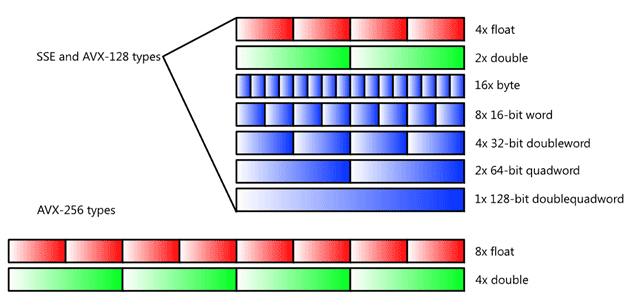
\includegraphics[width=.49\linewidth]{./resources/IntelISA/SSEAVXDataTypes}
% 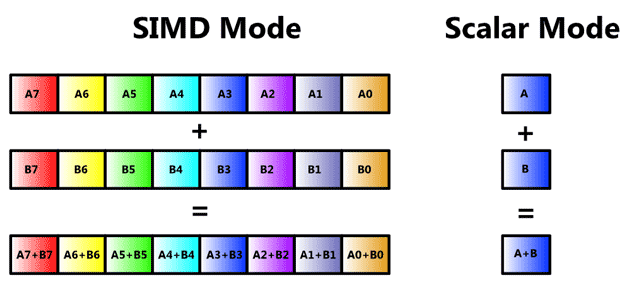
\includegraphics[width=.49\linewidth]{./resources/IntelISA/SIMD}

% \end{frame}

\hypertarget{background}{%
\section{Background}\label{background}}

\begin{frame}{Motivation of Vectorization}
\protect\hypertarget{motivation-of-vectorization}{}

\begin{block}{}

\begin{itemize}
    \item Modern processors exploit parallelism of all kinds to address the power wall issue.

    \item SIMD (Single Instruction, Multiple Data) operations leverages data parallelism to boost performance.
    
    %\visible<2->{
      \item Vectorization replaces homogeneous scalar operations with a set of SIMD arithmetic instructions in CPU.%}
\end{itemize}

\begin{figure}[htbp]
\centerline{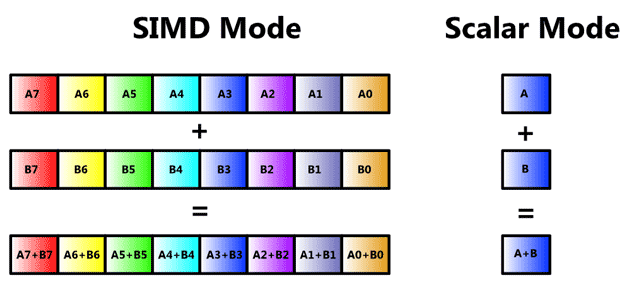
\includegraphics[width=0.45\textwidth]{./resources/IntelISA/SIMD.png}}
\caption{SIMD vs scalar operations.\textsuperscript{[9]}}
\end{figure}

\end{block}

\end{frame}

\begin{frame}{Intel Vector ISA}
\protect\hypertarget{intel-vectorization-isa}{}

\begin{block}{}

\begin{itemize}
  \item AVX2 expands vector register to 256 bits for most integer operations and supports FMA (fused multiply-accumulate) operations\textsuperscript{[10]}.
  \item The latest instruction set is AVX-512 and is available mostly in server and high-end desktop processors. 
  %\visible<2->{
  \item Vectorization scales the performance with vector bit width\textsuperscript{[9]}.
  \item Due to instruction execution and potential irregular memory access, \texttt{InsertElement} and \texttt{ExtractElement} incur extra cost.%}
\end{itemize}
\begin{figure}[htbp]
  \vspace{-20pt}
\centering
%<!--\subfloat[SIMD vs scalar operations.\label{fig:1a}]{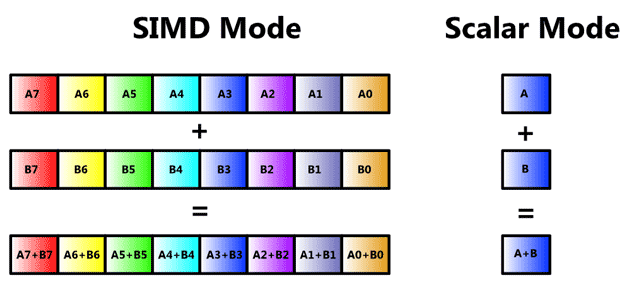
\includegraphics[width=0.45\textwidth]{./resources/IntelISA/SIMD.png}}\hfill\\-->
\subfloat[{Intel SSE and AVX data type.[9]\label{fig:1b}}] {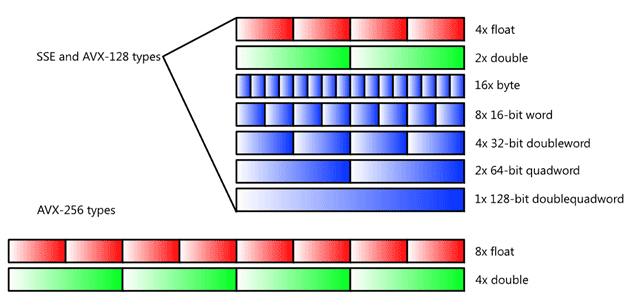
\includegraphics[width=0.45\textwidth]{./resources/IntelISA/SSEAVXDataTypes.png}}\hfill
\subfloat[{relative performance across sizes.[9]\label{fig:1c}}]{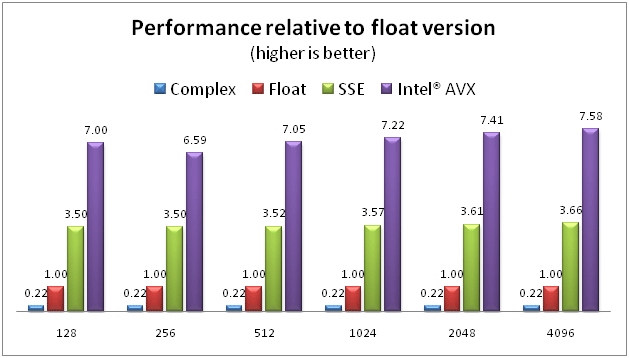
\includegraphics[width=0.5\textwidth]{./resources/IntelISA/RelativePerformance.png}}
%<!--\caption{General caption.}--> \label{fig:1}
\end{figure}

\end{block}

\end{frame}

\begin{frame}{Vectorizers in LLVM}
  \begin{block}{}
  \begin{itemize}
    \item LLVM vectorizers are IR to IR passes.
    \item They are target-independent, as they are before lowering!
    \item They transform \texttt{scalar} registers and operations into \texttt{vector} ones.
  \end{itemize}
  \end{block}
  %\pause
  \begin{block}{}
    \begin{itemize}
      \item SLP algorithm was proposed in 2000\textsuperscript{[4]}.
      \item GCC adpoted the loop-aware variant of SLP vectorizer\textsuperscript{[6]}.
      \item Later LLVM implemented SLP to complement its Loop Vectorizer.
      \item SLP Vectorizer immediately succeeds Loop Vectorizer in the optimization pipeline.
    \end{itemize}
  \end{block}
  %\pause
  \begin{block}{Programmers' hints are critical to vectorization and never ignored by LLVM.}
    \begin{itemize}
      \item \texttt{LoopVectorizeHints} reflects hints by \texttt{\#pragma}, e.g., vectorization width, unroll factor, force enabling.
      \item \texttt{!alias} metadata reflects \texttt{\_\_restrict} keyword.\textsuperscript{[12]}
    \end{itemize}
  \end{block}
\end{frame}

\hypertarget{algorithm}{%
\section{Bottom-Up SLP Algorithm}\label{algorithm}}


\begin{frame}{Bottom-Up SLP Vectorization}
  \begin{block}{}
  \begin{itemize}
    \item vectorizes straightforward code. It does not exploit or transform loop.
  \end{itemize}
\end{block}
\begin{block}{Steps}
  \begin{enumerate}
    \item builds the tree bottom-up, i.e., starting from the store instruction.
    \item traces the def-use chain to involve all possible bundles.
    \item scheduling: check cyclic memory dependency.
  \end{enumerate}
\end{block}
\begin{block}{Main challenges}
  \begin{itemize}
    \item determine consecutive access.
    \item determine cyclic memory dependency.
    \item handle all sorts of instructions.
  \end{itemize}
\end{block}
\begin{block}{}
  The following visualization is from Porpodas\textsuperscript{{[13]}}.
\end{block}

\end{frame}

\begin{frame}{}
\protect\hypertarget{section-2}{}

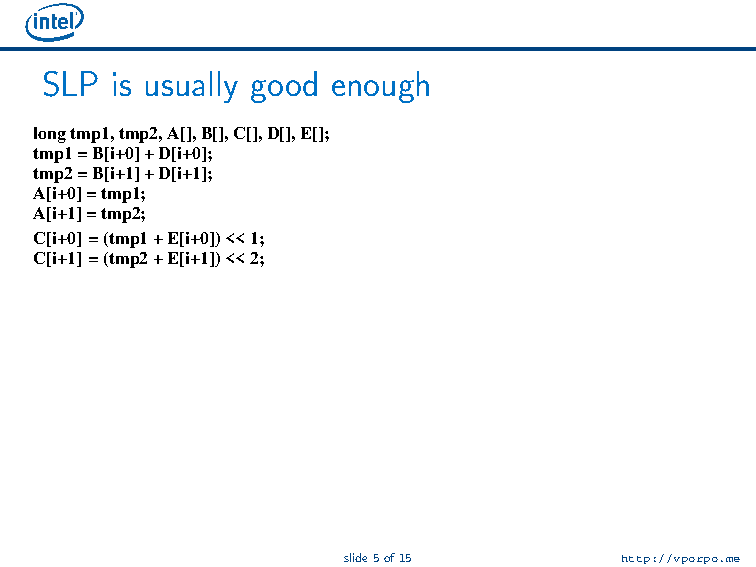
\includegraphics[width=0.9\textwidth,height=4.16667in]{./resources/SLPVisualization/Binder1-2.pdf}

\end{frame}

\begin{frame}{}
\protect\hypertarget{section-3}{}

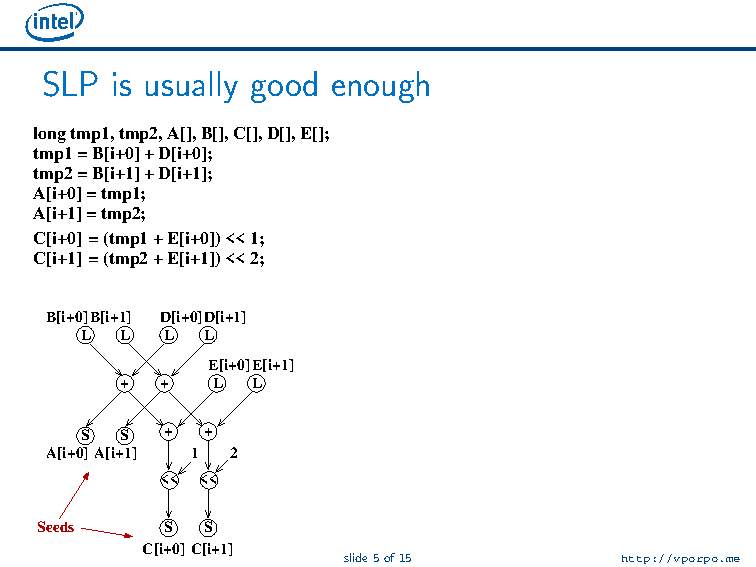
\includegraphics[width=0.9\textwidth,height=4.16667in]{./resources/SLPVisualization/Binder1-3.pdf}

\end{frame}

\begin{frame}{}
\protect\hypertarget{section-4}{}

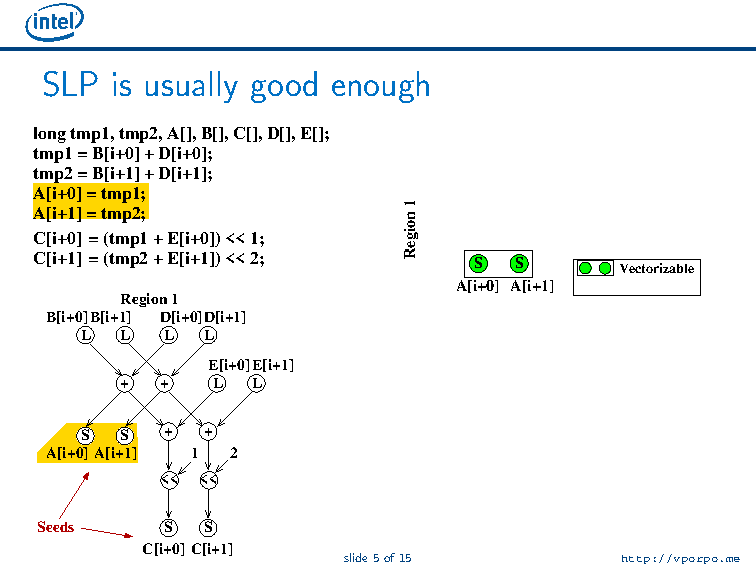
\includegraphics[width=0.9\textwidth,height=4.16667in]{./resources/SLPVisualization/Binder1-4.pdf}

\end{frame}

\begin{frame}{}
\protect\hypertarget{section-5}{}

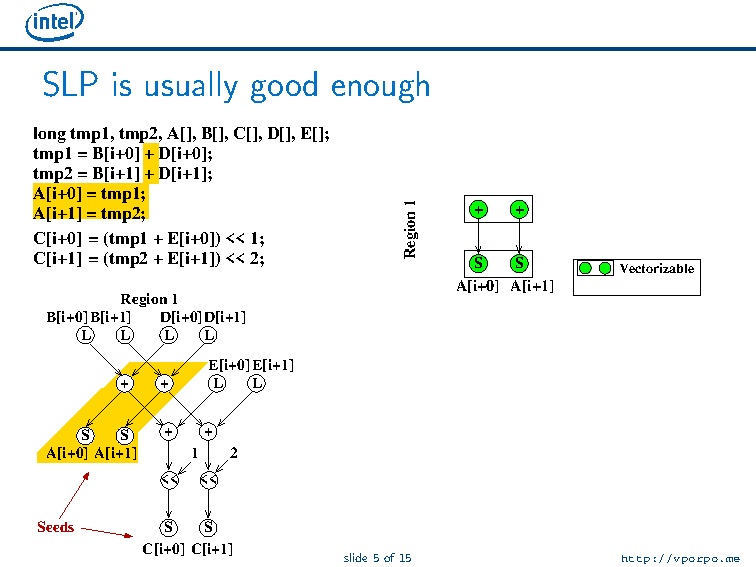
\includegraphics[width=0.9\textwidth,height=4.16667in]{./resources/SLPVisualization/Binder1-5.pdf}

\end{frame}

\begin{frame}{}
\protect\hypertarget{section-6}{}

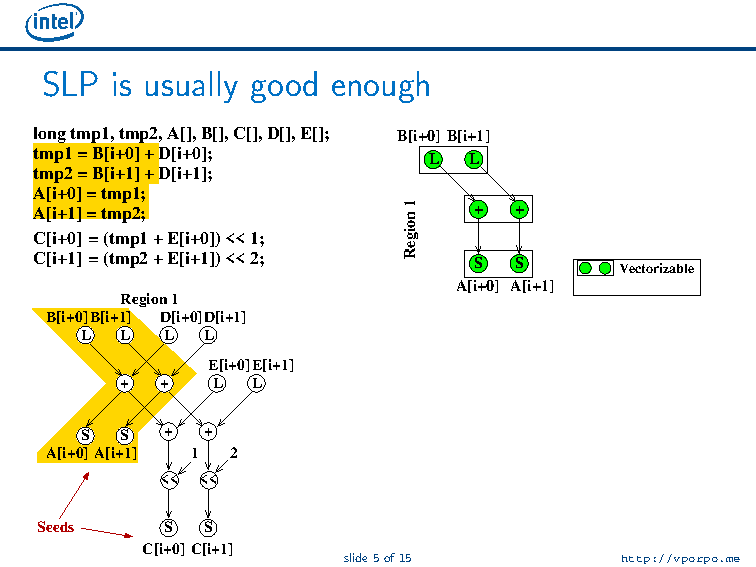
\includegraphics[width=0.9\textwidth,height=4.16667in]{./resources/SLPVisualization/Binder1-6.pdf}

\end{frame}

\begin{frame}{}
\protect\hypertarget{section-7}{}

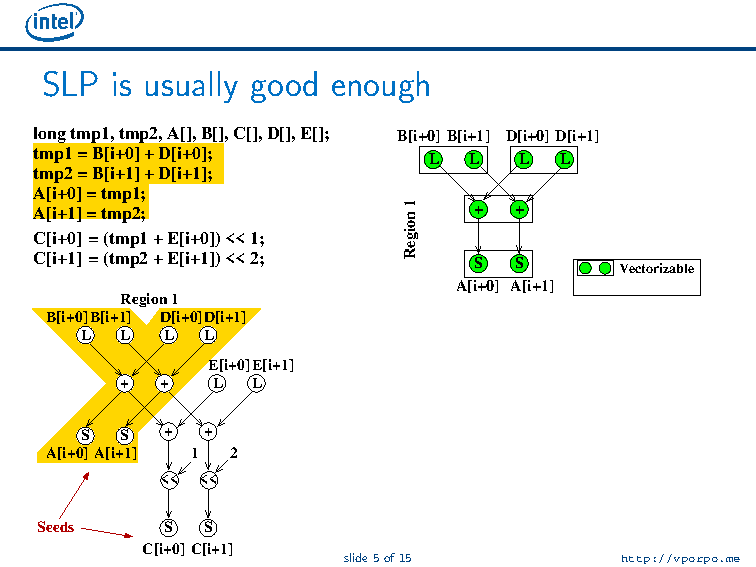
\includegraphics[width=0.9\textwidth,height=4.16667in]{./resources/SLPVisualization/Binder1-7.pdf}

\end{frame}

\begin{frame}{}
\protect\hypertarget{section-8}{}

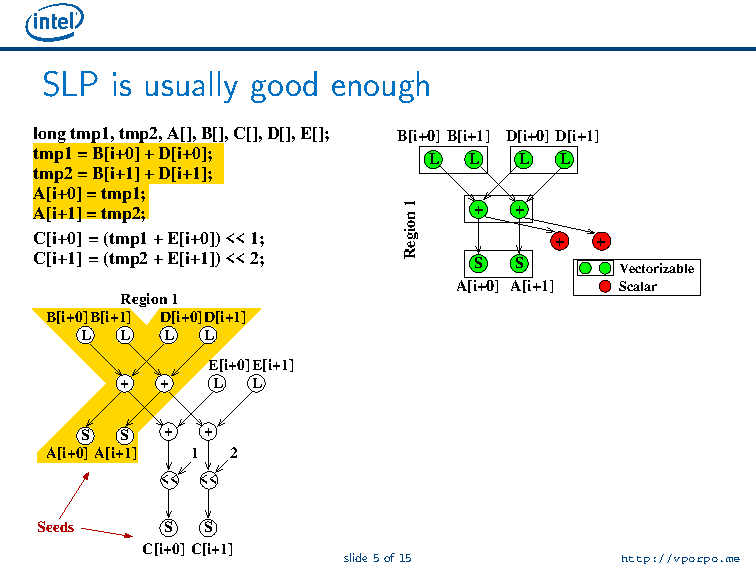
\includegraphics[width=0.9\textwidth,height=4.16667in]{./resources/SLPVisualization/Binder1-8.pdf}

\end{frame}

\begin{frame}{}
\protect\hypertarget{section-9}{}

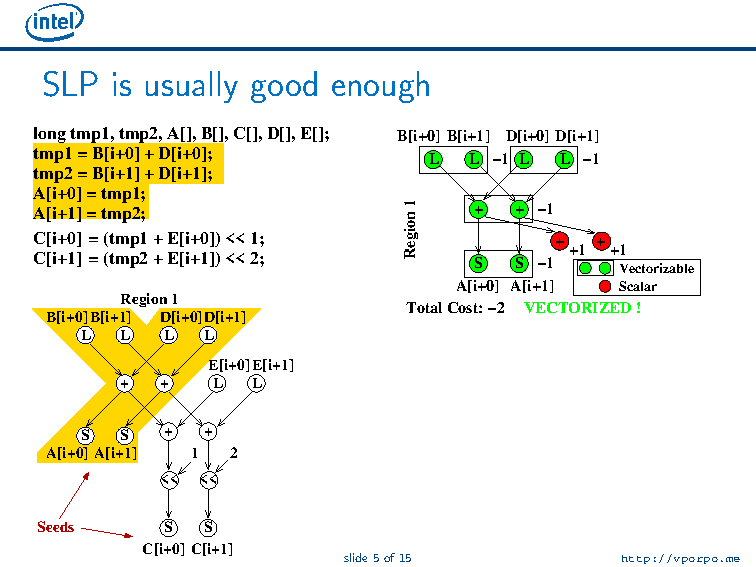
\includegraphics[width=0.9\textwidth,height=4.16667in]{./resources/SLPVisualization/Binder1-9.pdf}

\end{frame}

\begin{frame}{}
\protect\hypertarget{section-10}{}

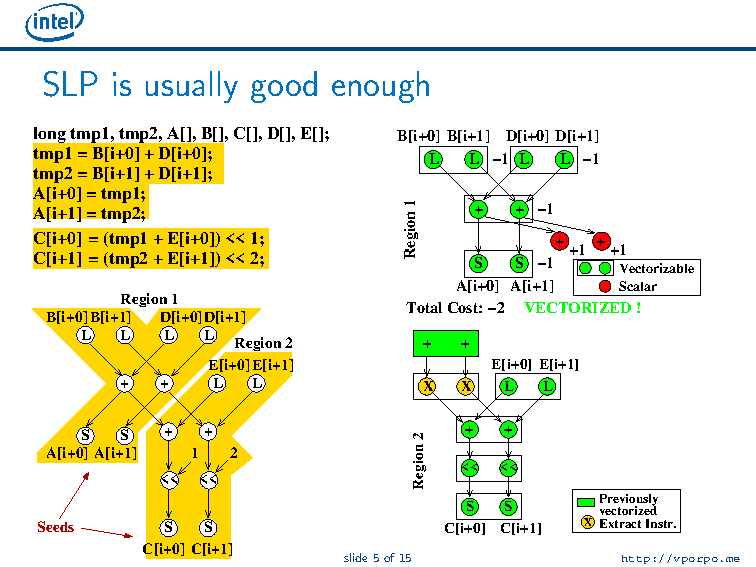
\includegraphics[width=0.9\textwidth,height=4.16667in]{./resources/SLPVisualization/Binder1-10.pdf}

\end{frame}

\begin{frame}{}
\protect\hypertarget{section-11}{}

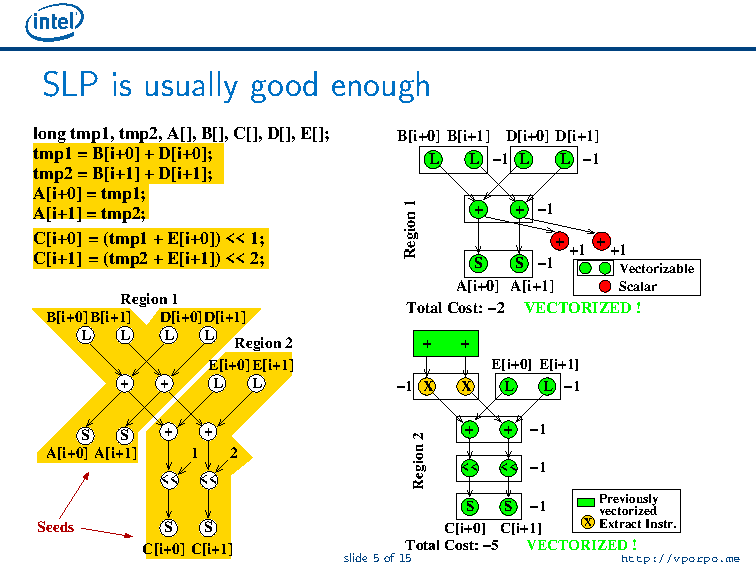
\includegraphics[width=0.9\textwidth,height=4.16667in]{./resources/SLPVisualization/Binder1-11.pdf}

\end{frame}

\begin{frame}{}
\protect\hypertarget{section-12}{}

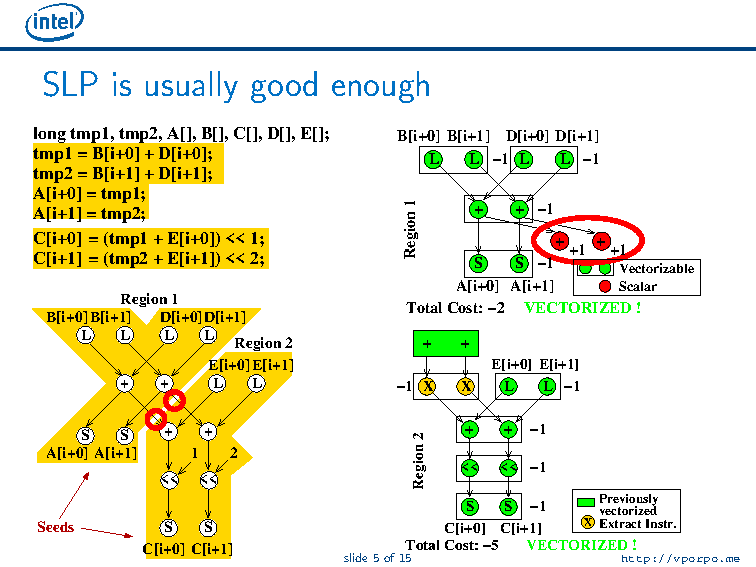
\includegraphics[width=0.9\textwidth,height=4.16667in]{./resources/SLPVisualization/Binder1-12.pdf}

\end{frame}

\begin{frame}{}
\protect\hypertarget{section-13}{}

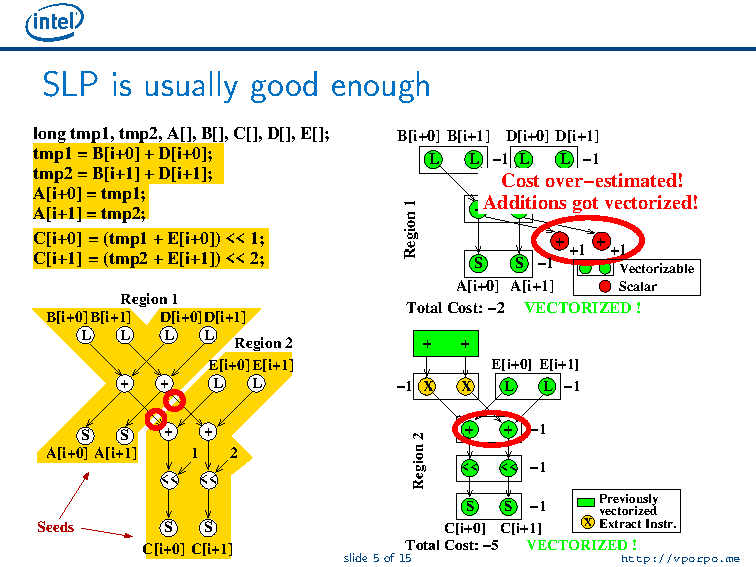
\includegraphics[width=0.9\textwidth,height=4.16667in]{./resources/SLPVisualization/Binder1-13.pdf}

\end{frame}

\begin{frame}{Bottom-Up SLP Vectorization}
  \begin{block}{}
  \begin{itemize}
    \item vectorizes straightforward code. It does not exploit or transform loop.
  \end{itemize}
\end{block}
\begin{block}{Steps}
  \begin{enumerate}
    \item builds the tree bottom-up, i.e., starting from the store instruction.
    \item traces the def-use chain to involve all possible bundles.
    \item scheduling: check cyclic memory dependency.
  \end{enumerate}
\end{block}
\begin{block}{Main challenges}
  \begin{itemize}
    \item determine consecutive access.
    \item determine cyclic memory dependency.
    \item handle all sorts of instructions.
  \end{itemize}
\end{block}
\end{frame}

\hypertarget{implementation}{%
\section{Implementation}\label{implementation}}



\begin{frame}{Nuances}
\protect\hypertarget{nuances}{}
\begin{block}{We implement the stem part of the algorithm}
  \begin{itemize}
  \item reduction is not supported.
  \item loop-awareness is not supported.
  \end{itemize}
  
\end{block}


\begin{block}{Instructions that we don't handle}
\begin{itemize}
  \item \texttt{ExtractValue}, \texttt{ExtractElement}: Reuse the vectorized bundle from previous trees.
  \item \texttt{GetElementPtr}: Pointer arithmetic complicates both consecutiveness and profitability determination.
  \item \texttt{PHI}: Inserts vectorized value at teminators of each incoming basic blocks.
  \item \texttt{Call}: Exploits LLVM intrinsics.
  \item \texttt{ShuffleVector}: Exploits alternate op sequence, e.g. \texttt{add}-\texttt{sub}.
  \item Commutative binary operators: Reordering may enable vectorization. 
\end{itemize}

\end{block}
\end{frame}


\begin{frame}{Nuances}
  \begin{block}{Infrastructure provided by analysis passes}

    \begin{itemize}
    \item \texttt{ScalarEvolution} helps analyze whether two load or two store locations are consecutive.
    \item \texttt{AliasAnalysis} detects memory dependency. 
    \item \texttt{Transforms/Utils/VectorUtils.h} provides metadata propagation functionality.
    \end{itemize}
  
  \end{block}
\end{frame}

\begin{frame}[fragile]{Example \texttt{\@sub\_v16i32()} from arith-sub.ll}
  \protect\hypertarget{anexample}{}
  \begin{exampleblock}{Before transformation}
    \begin{lstlisting}[basicstyle=\tiny,escapeinside={(*}{*)}]
%a0 = load i32, i32* GEP inbounds ([16 x i32], [16 x i32]* @a32, i32 0, i64 0 ), align 4
(*$\cdots$*)
%a15 = load i32, i32* GEP inbounds ([16 x i32], [16 x i32]* @a32, i32 0, i64 15 ), align 4
%b0 = load i32, i32* GEP inbounds ([16 x i32], [16 x i32]* @b32, i32 0, i64 0), align 4
(*$\cdots$*)
%b15 = load i32, i32* GEP inbounds ([16 x i32], [16 x i32]* @b32, i32 0, i64 15), align 4
%r0 = sub i32 %a0 , %b0
(*$\cdots$*)
%r15 = sub i32 %a15 , %b15
store i32 %r0 , i32* GEP inbounds ([16 x i32], [16 x i32]* @c32, i32 0, i64 0 ), align 4
(*$\cdots$*)
store i32 %r15 , i32* GEP inbounds ([16 x i32], [16 x i32]* @c32, i32 0, i64 15 ), align 4
    \end{lstlisting}
  \end{exampleblock}
  \begin{exampleblock}{After transformation}
      \begin{lstlisting}[basicstyle=\tiny,escapeinside={(*}{*)}]
%1 = load <16 x i32>, <16 x i32>* bitcast ([16 x i32]* @a32 to <16 x i32>*), align 4
%2 = load <16 x i32>, <16 x i32>* bitcast ([16 x i32]* @b32 to <16 x i32>*), align 4
%3 = sub <16 x i32> %1, %2
store <16 x i32> %3, <16 x i32>* bitcast ([16 x i32]* @c32 to <16 x i32>*), align 4
      \end{lstlisting}
    \end{exampleblock}
  \end{frame}
  
\hypertarget{pruning}{%
\section{Pruning the Tree for More Profit}\label{pruning}}

\begin{frame}{}
\begin{block}{Ideas from TSLP\textsuperscript{[5]}}
  \begin{itemize}
      \item Prunes the unprofitable subregion and not to vectorize them.
      \item Tries out many cuts, not all.
      \item Looks for the best cut.
  \end{itemize}
\end{block}
\begin{block}{What we did}
  \begin{itemize}
    \item We adopt these idea from TSLP\textsuperscript{[5]}.
    \item We search for the best cut of the tree-cluster and apply it before vectorization.
    \item We search for the best vectorization width.
    \item We copy from llvm-3.5.0 the handlers for unsupported instructions.
  \end{itemize}
\end{block}
\begin{block}{}
  The following visualization is from Porpodas and Jones\textsuperscript{{[5]}}.
\end{block}
\end{frame}


\begin{frame}{}
  \protect\hypertarget{section-14}{}
  
  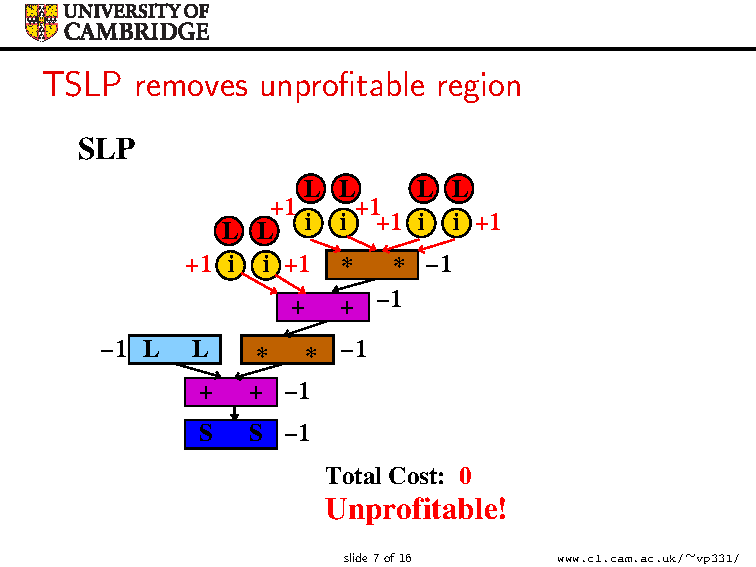
\includegraphics[width=0.9\textwidth,height=4.16667in]{./resources/TSLP/Porpodas-ThrottlingAutomaticVectorization-45.pdf}
  
  \end{frame}
  
  \begin{frame}{}
  \protect\hypertarget{section-15}{}
  
  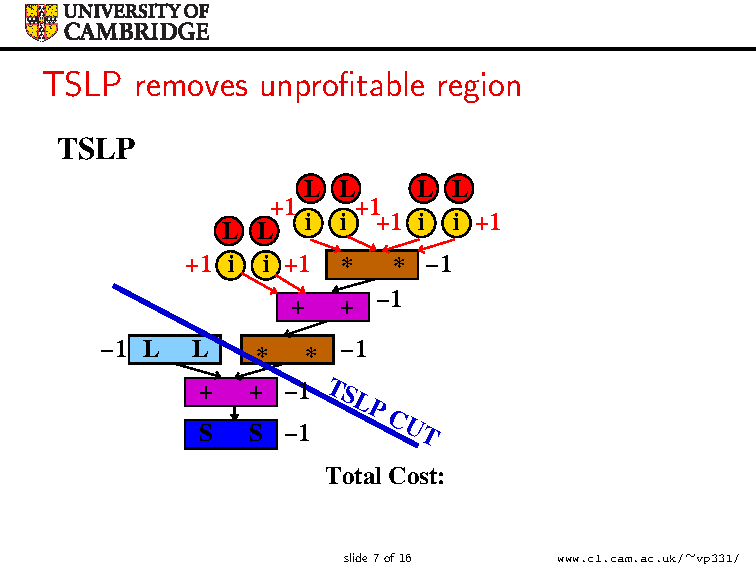
\includegraphics[width=0.9\textwidth,height=4.16667in]{./resources/TSLP/Porpodas-ThrottlingAutomaticVectorization-46.pdf}
  
  \end{frame}
  
  \begin{frame}{}
  \protect\hypertarget{section-16}{}
  
  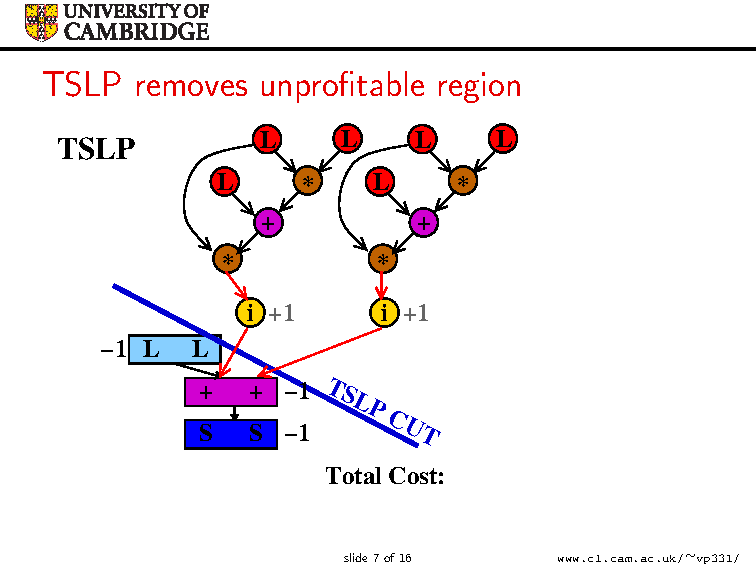
\includegraphics[width=0.9\textwidth,height=4.16667in]{./resources/TSLP/Porpodas-ThrottlingAutomaticVectorization-47.pdf}
  
  \end{frame}
  
  \begin{frame}{}
  \protect\hypertarget{section-17}{}
  
  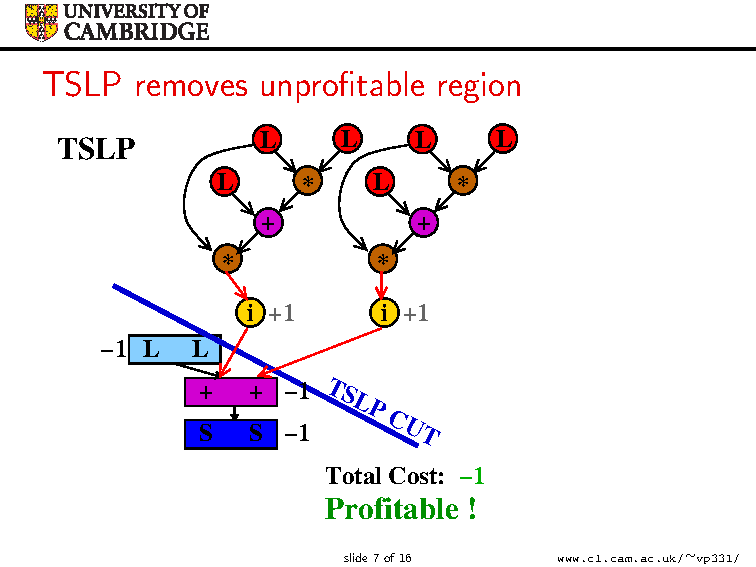
\includegraphics[width=0.9\textwidth,height=4.16667in]{./resources/TSLP/Porpodas-ThrottlingAutomaticVectorization-48.pdf}
  
  \end{frame}

  \begin{frame}{}
\begin{block}{Ideas from TSLP\textsuperscript{[5]}}
  \begin{itemize}
      \item Prunes the unprofitable subregion and not to vectorize them.
      \item Tries out many cuts, not all.
      \item Looks for the best cut.
  \end{itemize}
\end{block}
\begin{block}{What we did}
  \begin{itemize}
    \item We adopt these idea from TSLP\textsuperscript{[5]}.
    \item We search for the best cut of the tree-cluster and apply it before vectorization.
    \item We search for the best vectorization width.
    \item We copy from llvm-3.5.0 the handlers for unsupported instructions.
  \end{itemize}
\end{block}
\end{frame}

\hypertarget{Evaluation}{%
\section{Evaluation}\label{evaluation}}

\begin{frame}{Correctness Test}
\protect\hypertarget{correctness}{}
\begin{block}{Curated list of test cases from LLVM Repo.\textsuperscript{[14]}}
\begin{itemize}
\item Expected Passes : 4
\item Unexpected Failures: 18
\item Passed: \textcolor{green}{cmp\_sel.ll,
extract-shuffle.ll, load-bitcast-vec.ll, odd\_store.ll}
\item Failing: \textcolor{red}{arith-sub.ll, broadcast.ll,
cast.ll, commutativity.ll, different-vec-widths.ll, external\_user.ll,
external\_user\_jumbled\_load.ll, extract.ll, extractelement.ll,
jumbled-load-multiuse.ll, jumbled-load-shuffle-placement.ll,
jumbled-load-used-in-phi.ll, load-merge.ll, long\_chains.ll,
multi\_block.ll, multi\_user.ll, phi.ll, phi3.ll}
\end{itemize}
\end{block}
\end{frame}

\begin{frame}{Performance Evaluation}
\begin{block}{Scientific workload from OpenBenchmark\textsuperscript{[8]}}
\begin{itemize}
\item Single-threaded: SciMark 1.3.2, Himeno Benchmark 1.3.0
\item Pthread: C-Ray 1.2.0 
\item OpenMP: N-queens 1.2.1, Smallpt 1.2.1
\end{itemize}
\end{block}

\begin{block}{Test environment}
  \begin{itemize}
\item CPU: Intel(R) Core(TM) i9-9900K CPU @ 3.60GHz
\item Memory: 2x8GB @ 2133MHz
\item OS: CentOS-8 (1911)
\item Base LLVM version: 8.0.1
\item GCC version: 8.3.1
\item Intel OpenMP library version: 2020.1.217
  \end{itemize}
\end{block}
\end{frame}

\begin{frame}
\begin{block}{Methodology}
\begin{itemize}
\item Our pass is compared with the original SLP vectorizer from 8.0.1.
\item Two passes are compared in the O3 pipeline.
\item We dump and replicate the O3 optimization pipeline.
\item We replace the original \texttt{-slp-vectorizer} with \texttt{-slpvect-kdw}, in the form of shared library, to run our pass.
\end{itemize}
\end{block}

  \begin{figure}[htbp]
    \centerline{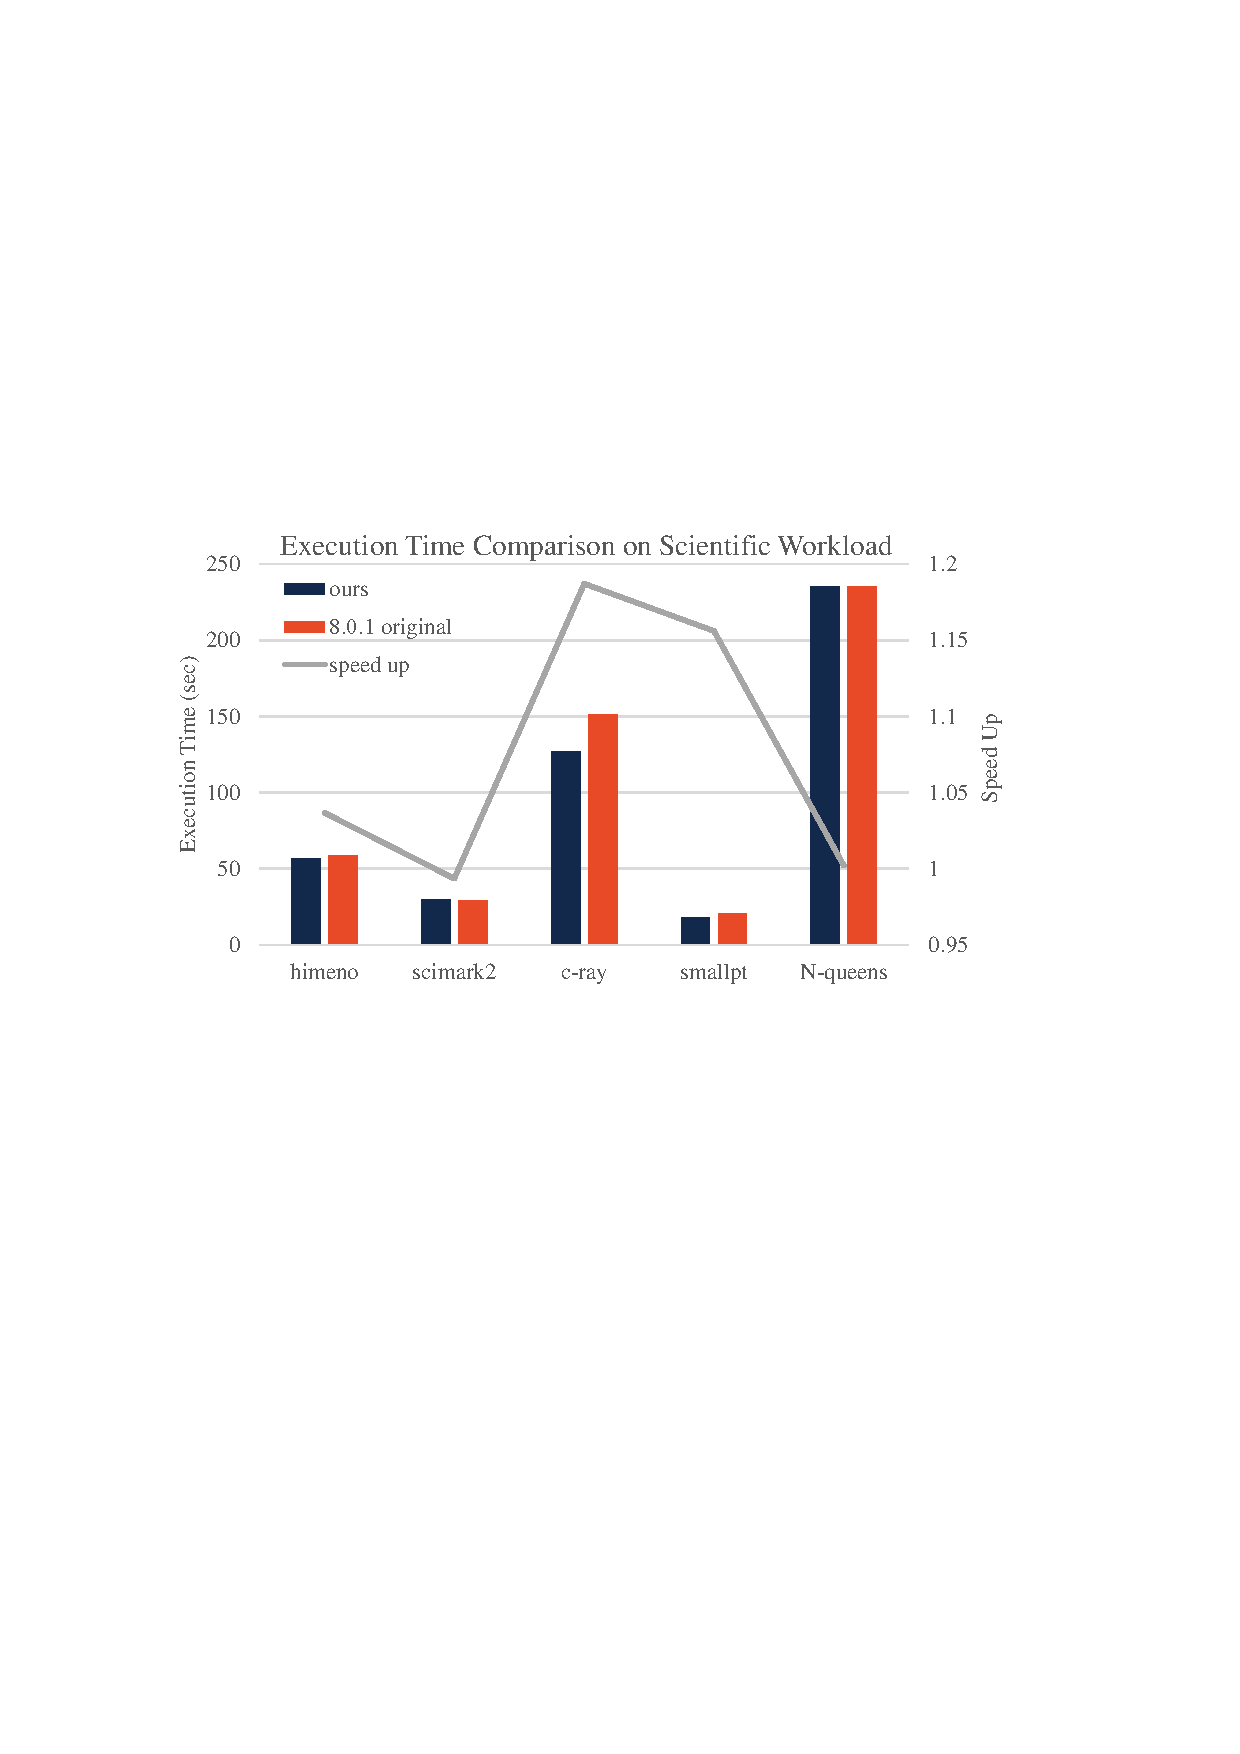
\includegraphics[width=0.75\textwidth]{./resources/Evaluation/figure.pdf}}
    %\caption{SIMD vs scalar operations.}
    \end{figure}

\end{frame}


\hypertarget{reference}{%
\section{Reference}\label{reference}}

\begin{frame}{Reference}
\protect\hypertarget{reference-1}{}

{[}1{]} Renato Golin. LLVM Auto-Vectorization: Past, Present and Future. \url{llvm.org/devmtg/2014-02/slides/golin-AutoVectorizationLLVM.pdf}

{[}2{]} Hal Finkel. Autovectorization with LLVM. \url{llvm.org/devmtg/2012-04-12/Slides/Hal_Finkel.pdf}

{[}3{]} Nadav Rotem and Arnold Schwaighofer. Vectorization in LLVM. \url{llvm.org/devmtg/2013-11/slides/Rotem-Vectorization.pdf}

{[}4{]} Samuel Larsen and Saman Amarasinghe. Exploiting Superword Level Parallelism with Multimedia Instruction Sets.

{[}5{]} Vasileios Porpodas and Timothy M. Jones. Throttling Automatic Vectorization: When Less Is More. \url{llvm.org/devmtg/2015-10/slides/Porpodas-ThrottlingAutomaticVectorization.pdf}

{[]}6{]} Ira Rosen et al. Loop-Aware SLP in GCC.

\end{frame}

\begin{frame}{Reference}
  \protect\hypertarget{reference-2}{}  
{[}7{]} Vasileios Porpodas et. al. Look-Ahead SLP: Auto-vectorization in the presence of commutative operations. \url{llvm.org/devmtg/2018-04/slides/Rocha-Look-Ahead\%20SLP.pdf}

{[}8{]} OpenBenchmark. OpenBenchmark Test on SLPVectorizer in LLVM 3.4. \url{openbenchmarking.org/result/1307291-SO-FSLPVECTO83}

{[}9{]} Intel. Introduction to Intel Advanced Vector Extensions. \url{software.intel.com/en-us/articles/introduction-to-intel-advanced-vector-extensions}

{[}10{]} Wikipedia. Advanced Vector Extensions. \url{en.wikipedia.org/wiki/Advanced_Vector_Extensions}

{[}11{]} Dan Gohman. Scalar Evolution and Loop Optimization \url{llvm.org/devmtg/2009-10/ScalarEvolutionAndLoopOptimization.pdf}

{[}12{]} Hal Finkel. Restrict-qualified pointers in LLVM. \url{llvm.org/devmtg/2017-02-04/Restrict-Qualified-Pointers-in-LLVM.pdf}

\end{frame}

\begin{frame}{Reference}
  \protect\hypertarget{reference-3}{}   
{[}13{]} Vasileios Porpodas. SuperGraph-SLP Auto-Vectorization. \url{vporpo.me/papers/sgslp_pact2017_slides.pdf}

{[}14{]} LLVM. Github: llvm-project/llvm/test/. \url{github.com/llvm/llvm-project/tree/master/llvm/test}
\end{frame}


\end{document}
